%%%%%%%%%%%%%%%%%%%%%%%%%%%%%%%%%%%%%%%%%%%%%%%%%%%%%%%%%%%%%%%
%% OXFORD THESIS TEMPLATE

% Use this template to produce a standard thesis that meets the Oxford University requirements for DPhil submission
%
% Originally by Keith A. Gillow (gillow@maths.ox.ac.uk), 1997
% Modified by Sam Evans (sam@samuelevansresearch.org), 2007
% Modified by John McManigle (john@oxfordechoes.com), 2015
% Modified by Ulrik Lyngs (ulrik.lyngs@cs.ox.ac.uk), 2018-, for use with R Markdown
%
% Ulrik Lyngs, 25 Nov 2018: Following John McManigle, broad permissions are granted to use, modify, and distribute this software
% as specified in the MIT License included in this distribution's LICENSE file.
%
% John commented this file extensively, so read through to see how to use the various options.  Remember that in LaTeX,
% any line starting with a % is NOT executed.

%%%%% PAGE LAYOUT
% The most common choices should be below.  You can also do other things, like replace "a4paper" with "letterpaper", etc.

% 'twoside' formats for two-sided binding (ie left and right pages have mirror margins; blank pages inserted where needed):
%\documentclass[a4paper,twoside]{templates/ociamthesis}
% Specifying nothing formats for one-sided binding (ie left margin > right margin; no extra blank pages):
%\documentclass[a4paper]{ociamthesis}
% 'nobind' formats for PDF output (ie equal margins, no extra blank pages):
%\documentclass[a4paper,nobind]{templates/ociamthesis}

% As you can see from the line below, oxforddown uses the a4paper size, 
% and passes in the binding option from the YAML header in index.Rmd:
\documentclass[a4paper, nobind]{templates/ociamthesis}


%%%%% ADDING LATEX PACKAGES
% add hyperref package with options from YAML %
\usepackage[pdfpagelabels]{hyperref}
% handle long urls
\usepackage{xurl}
% change the default coloring of links to something sensible
\usepackage{xcolor}

\definecolor{mylinkcolor}{RGB}{0,0,139}
\definecolor{myurlcolor}{RGB}{0,0,139}
\definecolor{mycitecolor}{RGB}{0,33,71}

\hypersetup{
  hidelinks,
  colorlinks,
  linktocpage=true,
  linkcolor=mylinkcolor,
  urlcolor=myurlcolor,
  citecolor=mycitecolor
}


% add float package to allow manual control of figure positioning %
\usepackage{float}

% enable strikethrough
\usepackage[normalem]{ulem}

% use soul package for correction highlighting
\usepackage{color, soulutf8}
\definecolor{correctioncolor}{HTML}{CCCCFF}
\sethlcolor{correctioncolor}
\newcommand{\ctext}[3][RGB]{%
  \begingroup
  \definecolor{hlcolor}{#1}{#2}\sethlcolor{hlcolor}%
  \hl{#3}%
  \endgroup
}
% stop soul from freaking out when it sees citation commands
\soulregister\ref7
\soulregister\cite7
\soulregister\citet7
\soulregister\autocite7
\soulregister\textcite7
\soulregister\pageref7

%%%%% FIXING / ADDING THINGS THAT'S SPECIAL TO R MARKDOWN'S USE OF LATEX TEMPLATES
% pandoc puts lists in 'tightlist' command when no space between bullet points in Rmd file,
% so we add this command to the template
\providecommand{\tightlist}{%
  \setlength{\itemsep}{0pt}\setlength{\parskip}{0pt}}
 
% allow us to include code blocks in shaded environments

% User-included things with header_includes or in_header will appear here
% kableExtra packages will appear here if you use library(kableExtra)
\usepackage{booktabs}
\usepackage{longtable}
\usepackage{array}
\usepackage{multirow}
\usepackage{wrapfig}
\usepackage{float}
\usepackage{colortbl}
\usepackage{pdflscape}
\usepackage{tabu}
\usepackage{threeparttable}
\usepackage{threeparttablex}
\usepackage[normalem]{ulem}
\usepackage{makecell}
\usepackage{xcolor}


%UL set section header spacing
\usepackage{titlesec}
% 
\titlespacing\subsubsection{0pt}{24pt plus 4pt minus 2pt}{0pt plus 2pt minus 2pt}


%UL set whitespace around verbatim environments
\usepackage{etoolbox}
\makeatletter
\preto{\@verbatim}{\topsep=0pt \partopsep=0pt }
\makeatother


%%%%%%% PAGE HEADERS AND FOOTERS %%%%%%%%%
\usepackage{fancyhdr}
\setlength{\headheight}{15pt}
\fancyhf{} % clear the header and footers
\pagestyle{fancy}
\renewcommand{\chaptermark}[1]{\markboth{\thechapter. #1}{\thechapter. #1}}
\renewcommand{\sectionmark}[1]{\markright{\thesection. #1}} 
\renewcommand{\headrulewidth}{0pt}

\fancyhead[LO]{\emph{\leftmark}} 
\fancyhead[RE]{\emph{\rightmark}} 




% UL page number position 
\fancyfoot[C]{\emph{\thepage}} %regular pages
\fancypagestyle{plain}{\fancyhf{}\fancyfoot[C]{\emph{\thepage}}} %chapter pages




%%%%% SELECT YOUR DRAFT OPTIONS
% This adds a "DRAFT" footer to every normal page.  (The first page of each chapter is not a "normal" page.)

% IP feb 2021: option to include line numbers in PDF

% for line wrapping in code blocks
\usepackage{fancyvrb}
\usepackage{fvextra}
\DefineVerbatimEnvironment{Highlighting}{Verbatim}{breaklines=true, breakanywhere=true, commandchars=\\\{\}}

% for quotations -- loaded here rather than in ociamthesis.cls, as it needs to
% be loaded after fvextra, otherwise we get a warning message
\usepackage{csquotes}

% This highlights (in blue) corrections marked with (for words) \mccorrect{blah} or (for whole
% paragraphs) \begin{mccorrection} . . . \end{mccorrection}.  This can be useful for sending a PDF of
% your corrected thesis to your examiners for review.  Turn it off, and the blue disappears.
\correctionstrue


%%%%% BIBLIOGRAPHY SETUP
% Note that your bibliography will require some tweaking depending on your department, preferred format, etc.
% If you've not used LaTeX before, I recommend just using pandoc for citations -- this is what's used unless you specific e.g. "citation_package: natbib" in index.Rmd
% If you're already a LaTeX pro and are used to natbib or something, modify as necessary.

% this allows the latex template to handle pandoc citations
\newlength{\cslhangindent}
\setlength{\cslhangindent}{1.5em}
\newlength{\csllabelwidth}
\setlength{\csllabelwidth}{3em}
\newlength{\cslentryspacingunit} % times entry-spacing
\setlength{\cslentryspacingunit}{\parskip}
\newenvironment{CSLReferences}[2] % #1 hanging-ident, #2 entry spacing
 {% don't indent paragraphs
  \setlength{\parindent}{0pt}
  % turn on hanging indent if param 1 is 1
  \ifodd #1
  \let\oldpar\par
  \def\par{\hangindent=\cslhangindent\oldpar}
  \fi
  % set entry spacing
  \setlength{\parskip}{1mm}
  \setlength{\baselineskip}{6mm}
 }%
 {}
\usepackage{calc}
\newcommand{\CSLBlock}[1]{#1\hfill\break}
\newcommand{\CSLLeftMargin}[1]{\parbox[t]{\csllabelwidth}{#1}}
\newcommand{\CSLRightInline}[1]{\parbox[t]{\linewidth - \csllabelwidth}{#1}\break}
\newcommand{\CSLIndent}[1]{\hspace{\cslhangindent}#1}




% Uncomment this if you want equation numbers per section (2.3.12), instead of per chapter (2.18):
%\numberwithin{equation}{subsection}


%%%%% THESIS / TITLE PAGE INFORMATION
% Everybody needs to complete the following:
\title{Integrative Analysis of Omics\\
Data with Biological Knowledge in\\
Translational Medicine}
\author{Ferran Briansó}
\college{Facultat de Biologia\\
Departament de Genètica, Microbiologia i Estadística}

% Master's candidates who require the alternate title page (with candidate number and word count)
% must also un-comment and complete the following three lines:

% Uncomment the following line if your degree also includes exams (eg most masters):
%\renewcommand{\submittedtext}{Submitted in partial completion of the}
% Your full degree name.  (But remember that DPhils aren't "in" anything.  They're just DPhils.)
\degree{Doctor of Philosophy}

% Term and year of submission, or date if your board requires (eg most masters)
\degreedate{XXXX XX 2023}


%%%%% YOUR OWN PERSONAL MACROS
% This is a good place to dump your own LaTeX macros as they come up.

% To make text superscripts shortcuts
\renewcommand{\th}{\textsuperscript{th}} % ex: I won 4\th place
\newcommand{\nd}{\textsuperscript{nd}}
\renewcommand{\st}{\textsuperscript{st}}
\newcommand{\rd}{\textsuperscript{rd}}

%%%%% THE ACTUAL DOCUMENT STARTS HERE
\begin{document}

%%%%% CHOOSE YOUR LINE SPACING HERE
% This is the official option.  Use it for your submission copy and library copy:
\setlength{\textbaselineskip}{22pt plus2pt}
% This is closer spacing (about 1.5-spaced) that you might prefer for your personal copies:
%\setlength{\textbaselineskip}{18pt plus2pt minus1pt}

% You can set the spacing here for the roman-numbered pages (acknowledgements, table of contents, etc.)
\setlength{\frontmatterbaselineskip}{17pt plus1pt minus1pt}

% UL: You can set the line and paragraph spacing here for the separate abstract page to be handed in to Examination schools
\setlength{\abstractseparatelineskip}{13pt plus1pt minus1pt}
\setlength{\abstractseparateparskip}{0pt plus 1pt}

% UL: You can set the general paragraph spacing here - I've set it to 2pt (was 0) so
% it's less claustrophobic
\setlength{\parskip}{2pt plus 1pt}

%
% Customise title page
%
\def\crest{{\includegraphics[width=8cm]{templates/logo\_UBblanc.png}}}
\renewcommand{\university}{Universitat de Barcelona}
\renewcommand{\submittedtext}{A thesis submitted for the degree of}
\renewcommand{\thesistitlesize}{\fontsize{22pt}{28pt}\selectfont}
\renewcommand{\gapbeforecrest}{25mm}
\renewcommand{\gapaftercrest}{25mm
}


% Leave this line alone; it gets things started for the real document.
\setlength{\baselineskip}{\textbaselineskip}


%%%%% CHOOSE YOUR SECTION NUMBERING DEPTH HERE
% You have two choices.  First, how far down are sections numbered?  (Below that, they're named but
% don't get numbers.)  Second, what level of section appears in the table of contents?  These don't have
% to match: you can have numbered sections that don't show up in the ToC, or unnumbered sections that
% do.  Throughout, 0 = chapter; 1 = section; 2 = subsection; 3 = subsubsection, 4 = paragraph...

% The level that gets a number:
\setcounter{secnumdepth}{2}
% The level that shows up in the ToC:
\setcounter{tocdepth}{1}


%%%%% ABSTRACT SEPARATE
% This is used to create the separate, one-page abstract that you are required to hand into the Exam
% Schools.  You can comment it out to generate a PDF for printing or whatnot.

% JEM: Pages are roman numbered from here, though page numbers are invisible until ToC.  This is in
% keeping with most typesetting conventions.
\begin{romanpages}

% Title page is created here
\maketitle

%%%%% DEDICATION
\begin{dedication}
  For XXXXX XXXXXX
\end{dedication}

%%%%% ACKNOWLEDGEMENTS


\begin{acknowledgements}
 	\ldots{} \ldots{} \ldots{} \ldots{}

 \begin{flushright}
 Ferran Brianso \\
 Mataro, BCN \\
 XX XXXXXX 2023
 \end{flushright}
\end{acknowledgements}



%%%%% ABSTRACT


\renewcommand{\abstracttitle}{Abstract}
\begin{abstract}
	The general concept of Data Integration can be defined as the combination of data residing in different sources in order to provide the users with a unified view of these data {[}1{]}. However, the practical meaning of the term Integration may vary from, for instance, the computational combination of data, to the combination of studies performed independently, the simultaneous analysis of multiple variables on multiple datasets, or any possible approach for homogeneously querying heterogeneous data sources. Therefore, in many cases, an integrative analysis may be preferable than a simple combination of data from distinct sources. Integrative analysis allows not only for the combination of heterogeneous data, but also for the combined use of these data in order to get the most relevant information and, what is better, to be able to extract some information that could not be unveiled by the separated analysis of each of the original data types.

Over the past decade, advancements in omics technologies have facilitated the high-throughput monitoring of molecular and organism processes. These techniques have been widely applied to identify biological agents and to characterize biochemical systems, often focusing on the discovery of therapeutic targets and biomarkers related with specific diseases {[}2,3,4{]}. While many single-omic approaches target comprehensive analysis of genes (genomics), mRNA (transcriptomics), proteins (proteomics), and metabolites (metabolomics) among other, there is still field to improve omics data analyses through integrative methods {[}5,6{]}. In this sense, the integrative point of view defined in the paragraph above, applied to multi-omics data, is a promising approach to achieve better biomarker development in biomedical research projects, and this is the core idea of this work.

As the field of omics has evolved from analyzing a unique type of data to multiple types, it has been natural to extend the previous use of multivariate techniques to this new situation. With this aim classical and new multivariate techniques have been applied to the analysis of multi-omics datasets. Many of these techniques are dimension reduction methods that aim at finding main sources of variability in the data while maximizing some information characteristic such as the variance of each dataset, the correlation between groups of variables or other. Examples of such techniques are well consolidated methods such as Principal Component Analysis (PCA), Singular Value Decomposition (SVD), Correspondence Analysis (CA), and Partial Least Squares (PLS). Besides these more ``novel'' approaches have been used such as: Principal Components Regression, Coinertia and Multiple Coinertia Analysis, Generalized SVD, Sparse PLS, Multiple Factor Analysis (MFA), or combined versions of them {[}7,8,9{]}. Meng {[}10{]}, Cavill {[}11{]}, Wu {[}12{]}, Subramanian {[}30{]}, Krassowski {[}31{]}, and Cantini {[}32{]}, are good reviews of the state of the art of using multivariate and joint reduction methods for Integrative Multi-Omics Analysis.

Dimension reduction methods, especially those that are able to deal with situations that are typical from the omics context (with many more variables than samples, or possibly sparse matrices with many missing values), have been of great help in visualizing datasets or even for performing variable selection to find biomarkers for a given situation {[}12{]}. There is however one point where they underperform other approaches, that is, the difficulty in interpreting results from a biological point of view. This is relatively reasonable, because the most of these methods work by creating new variables that are some type of linear combination from the original ones. While this is useful, for example, for removing redundancy, this does not provide any clues on what these new dimensions may mean from a biological point of view.

This problem has been known since the beginning of using multivariate methods with omics data, but only a few approaches have been taken to deal with this. The first attempts to introduce biological information in the analyses consisted of using the most well-known database of biological functions, the Gene Ontology (GO) {[}13{]}. Fellenberg {[}14{]} introduces a way to integrate Gene Ontology information with Correspondence Analysis to facilitate the interpretation of microarray data. De Tayrac et al.~{[}15{]} applies multiple factor analysis to the integrative analysis of microarray and DNA copy number data. They apply GO Terms on data visualizations by treating these terms as supplemental information. In recent years the representation of biological knowledge has shifted from Gene Ontology to using Gene Sets {[}16{]}. Meng and Culhane {[}10{]} have introduced the Integrative Clustering with Gene Set Analysis where gene set expression analysis is performed based on multiple omics data; and Tyekucheva et al.~{[}17{]}, go one step further and use the results of Gene Set Expression Analysis (GSEA) to integrate different omics data.

Altogether, the previous approaches show several things: Although the idea that integrating quantitative data with biological knowledge may increase interpretability, the number of successful attempts to do this is still small. In this thesis, the use of either classical GO Terms or more flexible annotations (Gene Sets or custom annotations), will be combined with different approaches, and combinations of them if needed, to guide integrative analysis and to improve its biological interpretability from the point of view of the biomedical researchers.
\end{abstract}



%%%%% MINI TABLES
% This lays the groundwork for per-chapter, mini tables of contents.  Comment the following line
% (and remove \minitoc from the chapter files) if you don't want this.  Un-comment either of the
% next two lines if you want a per-chapter list of figures or tables.
\dominitoc % include a mini table of contents

% This aligns the bottom of the text of each page.  It generally makes things look better.
\flushbottom

% This is where the whole-document ToC appears:
\tableofcontents

\listoffigures
	\mtcaddchapter
  	% \mtcaddchapter is needed when adding a non-chapter (but chapter-like) entity to avoid confusing minitoc

% Uncomment to generate a list of tables:
\listoftables
  \mtcaddchapter
%%%%% LIST OF ABBREVIATIONS
% This example includes a list of abbreviations.  Look at text/abbreviations.tex to see how that file is
% formatted.  The template can handle any kind of list though, so this might be a good place for a
% glossary, etc.
% First parameter can be changed eg to "Glossary" or something.
% Second parameter is the max length of bold terms.
\begin{mclistof}{List of Abbreviations}{3.2cm}

\item[1-D, 2-D]

One- or two-dimensional, referring \textbf{in this thesis} to spatial dimensions in an image.

\item[Otter]

One of the finest of water mammals.

\item[Hedgehog]

Quite a nice prickly friend.

\end{mclistof} 


% The Roman pages, like the Roman Empire, must come to its inevitable close.
\end{romanpages}

%%%%% CHAPTERS
% Add or remove any chapters you'd like here, by file name (excluding '.tex'):
\flushbottom

% all your chapters and appendices will appear here
\hypertarget{intro}{%
\chapter{Introduction}\label{intro}}

\chaptermark{Introduction}

\minitoc 

\hypertarget{content-of-the-introductory-text-wip}{%
\section{Content of the introductory text (WIP)}\label{content-of-the-introductory-text-wip}}

The general concept of Data Integration can be defined as the combination of data residing in different sources in order to provide the users with a unified view of these data {[}1{]}. However, the practical meaning of the term Integration may vary from, for instance, the computational combination of data, to the combination of studies performed independently, the simultaneous analysis of multiple variables on multiple datasets, or any possible approach for homogeneously querying heterogeneous data sources. Therefore, in many cases, an integrative analysis may be preferable than a simple combination of data from distinct sources. Integrative analysis allows not only for the combination of heterogeneous data, but also for the combined use of these data in order to get the most relevant information and, what is better, to be able to extract some information that could not be unveiled by the separated analysis of each of the original data types.

Over the past decade, advancements in omics technologies have facilitated the high-throughput monitoring of molecular and organism processes. These techniques have been widely applied to identify biological agents and to characterize biochemical systems, often focusing on the discovery of therapeutic targets and biomarkers related with specific diseases {[}2,3,4{]}. While many single-omic approaches target comprehensive analysis of genes (genomics), mRNA (transcriptomics), proteins (proteomics), and metabolites (metabolomics) among other, there is still field to improve omics data analyses through integrative methods {[}5,6{]}. In this sense, the integrative point of view defined in the paragraph above, applied to multi-omics data, is a promising approach to achieve better biomarker development in biomedical research projects, and this is the core idea of this work.

As the field of omics has evolved from analyzing a unique type of data to multiple types, it has been natural to extend the previous use of multivariate techniques to this new situation. With this aim classical and new multivariate techniques have been applied to the analysis of multi-omics datasets. Many of these techniques are dimension reduction methods that aim at finding main sources of variability in the data while maximizing some information characteristic such as the variance of each dataset, the correlation between groups of variables or other. Examples of such techniques are well consolidated methods such as Principal Component Analysis (PCA), Singular Value Decomposition (SVD), Correspondence Analysis (CA), and Partial Least Squares (PLS). Besides these more ``novel'' approaches have been used such as: Principal Components Regression, Coinertia and Multiple Coinertia Analysis, Generalized SVD, Sparse PLS, Multiple Factor Analysis (MFA), or combined versions of them {[}7,8,9{]}. Meng (\protect\hyperlink{ref-meng_dimension_2016}{Meng et al., 2016}), Cavill (\protect\hyperlink{ref-cavill_transcriptomic_2016}{Cavill et al., 2016}), Wu {[}12{]}, Subramanian {[}30{]}, Krassowski {[}31{]}, and Cantini {[}32{]}, are good reviews of the state of the art of using multivariate and joint reduction methods for Integrative Multi-Omics Analysis.

Dimension reduction methods, especially those that are able to deal with situations that are typical from the omics context (with many more variables than samples, or possibly sparse matrices with many missing values), have been of great help in visualizing datasets or even for performing variable selection to find biomarkers for a given situation {[}12{]}. There is however one point where they underperform other approaches, that is, the difficulty in interpreting results from a biological point of view. This is relatively reasonable, because the most of these methods work by creating new variables that are some type of linear combination from the original ones. While this is useful, for example, for removing redundancy, this does not provide any clues on what these new dimensions may mean from a biological point of view.

This problem has been known since the beginning of using multivariate methods with omics data, but only a few approaches have been taken to deal with this. The first attempts to introduce biological information in the analyses consisted of using the most well-known database of biological functions, the Gene Ontology (GO) {[}13{]}. Fellenberg {[}14{]} introduces a way to integrate Gene Ontology information with Correspondence Analysis to facilitate the interpretation of microarray data. De Tayrac et al. (\protect\hyperlink{ref-de_tayrac_simultaneous_2009}{Tayrac et al., 2009}) applies multiple factor analysis to the integrative analysis of microarray and DNA copy number data. They apply GO Terms on data visualizations by treating these terms as supplemental information. In recent years the representation of biological knowledge has shifted from Gene Ontology to using Gene Sets {[}16{]}. Meng and Culhane {[}10{]} have introduced the Integrative Clustering with Gene Set Analysis where gene set expression analysis is performed based on multiple omics data; and Tyekucheva et al.~{[}17{]}, go one step further and use the results of Gene Set Expression Analysis (GSEA) to integrate different omics data.

Altogether, the previous approaches show several things: Although the idea that integrating quantitative data with biological knowledge may increase interpretability, the number of successful attempts to do this is still small. In this thesis, the use of either classical GO Terms or more flexible annotations (Gene Sets or custom annotations), will be combined with different approaches, and combinations of them if needed, to guide integrative analysis and to improve its biological interpretability from the point of view of the biomedical researchers.

\hypertarget{backgroundstate-of-the-art}{%
\section{Background/State of the Art}\label{backgroundstate-of-the-art}}

Falta desenvolupar punts

\hypertarget{omics-data-analyses}{%
\subsection{Omics data analyses}\label{omics-data-analyses}}

3 problemes esencials (veure projecte recerca Alex):

\begin{itemize}
\item
  \textbf{Omics data may be partly incomplete}, especially in multiomics studies, where not all types of data are usually available for all individuals.
\item
  \textbf{The results of these analyses are difficult to interpret}. If we agree that the ultimate goal of many analyzes is a better understanding of the underlying biological processes, for example, in a disease study context, it should be possible to establish a clear relationship between the outcome of an analysis and what this means biologically. And this is not always so.
\item
  \textbf{These kind of data analytics are difficult to standardize}, as it is not easy to make complex pipelines of multi-omics analyses, which integrate multiple processes with multiple sources, easy to reproduce or communicate.
\end{itemize}

Més el problema de la p\textgreater\textgreater n (Dimensionallity Reduction Techniques; The p\textgreater\textgreater n situation)

\hypertarget{the-problem-of-having-partly-incomplete-data}{%
\subsection{The problem of having partly incomplete data}\label{the-problem-of-having-partly-incomplete-data}}

Having partly incomplete data is a common challenge in biomedical multi-omics data analyses, where not all omics layers or samples have complete measurements for all variables of interest. This problem, known as missing data, can hinder the integrative analysis and interpretation of multi-omics datasets. Here, I will explain the issue of incomplete data in this context and provide relevant bibliographic references.

\textbf{Missing Data Types}: Missing data can occur in various forms in multi-omics datasets. For example, some omics layers may have missing values for certain variables (e.g., genes, proteins, metabolites), or specific samples may be missing data for certain omics layers. This can result from technical limitations, experimental design, or inherent biological variability. Reference: Kim, S., et al.~(2018). A survey of statistical methods for handling missing omics data. Statistical Methods in Medical Research, 27(10), 3026-3042.

\textbf{Impact on Analysis}: Incomplete data can introduce biases and distort the results of multi-omics analyses. It can affect downstream statistical analyses, clustering, network inference, and machine learning algorithms, leading to inaccurate or unreliable findings. Addressing missing data appropriately is crucial for obtaining valid and meaningful results. Reference: Tan, A., et al.~(2019). Handling missing omics data with advanced imputation techniques: A review. Journal of Integrative Bioinformatics, 16(2), 20180062.

\textbf{Missing Data Mechanisms}: Understanding the underlying mechanisms of missing data is essential for selecting appropriate imputation methods. Missing data can occur due to different mechanisms, such as missing completely at random (MCAR), missing at random (MAR), or missing not at random (MNAR). These mechanisms influence the choice of imputation techniques and the assumptions made during data analysis. Reference: Little, R. J. A., \& Rubin, D. B. (2002). Statistical analysis with missing data. Wiley Online Library.

\textbf{Imputation Methods}: Imputation techniques are employed to estimate missing values in multi-omics datasets. Various imputation methods, including mean imputation, regression imputation, multiple imputation, and machine learning-based approaches, have been proposed to handle missing data in different omics layers. Each method has its assumptions, strengths, and limitations, and the choice of imputation strategy should be carefully considered. Reference: Buuren, S. V., \& Groothuis-Oudshoorn, K. (2011). mice: Multivariate imputation by chained equations in R. Journal of Statistical Software, 45(3), 1-67.

\textbf{Uncertainty and Sensitivity Analysis}: Dealing with missing data introduces uncertainty in the imputed values and subsequent analyses. Sensitivity analyses, such as multiple imputation and bootstrapping, can help assess the robustness of the results to missing data assumptions and imputation methods. Reference: Sterne, J. A., et al.~(2009). Multiple imputation for missing data in epidemiological and clinical research: Potential and pitfalls. BMJ, 338, b2393.

Addressing the issue of incomplete data in multi-omics analyses is crucial to avoid biased or misleading results. By utilizing appropriate imputation methods and understanding the missing data mechanisms, researchers can mitigate the impact of missing data and enhance the accuracy and reliability of their analyses.

\hypertarget{results-interpretation-in-the-context-of-integrative-multi-omics-data-analyses}{%
\subsection{Results interpretation in the context of integrative multi-omics data analyses}\label{results-interpretation-in-the-context-of-integrative-multi-omics-data-analyses}}

Interpretation of results in integrative multi-omics data analyses is a critical challenge due to the complexity and high dimensionality of the data, as well as the need to integrate information from multiple omics layers. Here, I will explain the problem of result interpretation in this context and provide relevant bibliographic references.

\textbf{Data Integration Challenges}: Integrating multi-omics data involves combining information from different molecular layers such as genomics, transcriptomics, proteomics, and metabolomics. Each omics layer provides a unique perspective on biological processes, and integrating these layers can reveal comprehensive insights. However, interpreting the integrated results becomes challenging due to the heterogeneity and scale differences among the omics data. Reference: Wang, X., \& Zhang, B. (2018). Integrating multiple `omics' data for biomarker discovery and clinical assessment. Molecular \& Cellular Proteomics, 17(6), 991-1003.

\textbf{Dimensionality and Complexity}: Multi-omics data analyses often result in high-dimensional datasets with numerous features, making it difficult to interpret the results directly. The challenge lies in identifying the most relevant features or patterns and extracting meaningful biological insights from the vast amount of data. Reference: Nguyen, T. M., et al.~(2019). Integrative analysis of multi-omics data for discovery and functional studies of complex human diseases. Advances in Genetics, 103, 143-175.

\textbf{Contextual Interpretation}: Interpreting multi-omics results requires considering the biological context, such as pathways, networks, and regulatory interactions. Understanding how different omics layers interact and influence each other within biological systems is crucial for accurate interpretation. Reference: Mei, H., et al.~(2017). The road beyond omics: Integration of multi-omics data for the inference of regulatory networks and precision medicine. Computational and Structural Biotechnology Journal, 15, 359-366.

\textbf{Validation and Biological Significance}: Integrative multi-omics analyses often generate numerous associations, correlations, or biomarkers. However, validating and determining the biological significance of these findings is a key challenge. Experimental validation, functional enrichment analysis, and comparison with existing knowledge are essential for confirming the biological relevance of the results. Reference: Sun, H., et al.~(2020). Strategies for interpreting multi-omics studies in schizophrenia and other neuropsychiatric disorders. Journal of Psychiatric Research, 129, 121-133.

\textbf{Visualization and Interactive Tools}: Visualizing and exploring multi-omics data can aid in result interpretation. Interactive visualization tools that integrate different omics layers, provide network views, and enable user-driven exploration can facilitate the interpretation process. Reference: Swatloski, T., \& et al.~(2020). Multi-Omics Data Integration, Interpretation, and Its Application. Genes, 11(10), 1162.

In summary, the problem of result interpretation in integrative multi-omics data analyses stems from the challenges of data integration, high dimensionality, contextual understanding, validation, and visual exploration. Addressing these challenges requires a combination of statistical methods, biological knowledge, and interactive tools to extract meaningful insights from the integrated data.

\hypertarget{approaches-for-the-biological-and-clinical-interpretation}{%
\subsection{Approaches for the biological and clinical interpretation}\label{approaches-for-the-biological-and-clinical-interpretation}}

The biological and clinical interpretation of multi-omics data analysis results is crucial for gaining insights into the underlying molecular mechanisms, identifying biomarkers, and understanding disease processes.

\begin{enumerate}
\def\labelenumi{\arabic{enumi}.}
\item
  \textbf{Pathway and Functional Enrichment Analysis}: Pathway and functional enrichment analysis aim to identify overrepresented biological pathways, gene sets, or functional categories that are significantly associated with the differentially expressed genes or other omics features. These analyses help in understanding the biological processes, molecular functions, and cellular components that are affected in a particular condition or disease. Citation: Khatri, P., et al.~(2012). Ten years of pathway analysis: Current approaches and outstanding challenges. PLoS Computational Biology, 8(2), e1002375.
\item
  \textbf{Network Analysis}: Network analysis involves the construction and analysis of biological networks, such as gene regulatory networks or protein-protein interaction networks, using multi-omics data. Network-based approaches help in identifying key hub genes, modules, or subnetworks that play important roles in disease progression or phenotype. Citation: Barabási, A. L., et al.~(2011). Network medicine: A network-based approach to human disease. Nature Reviews Genetics, 12(1), 56-68.
\item
  \textbf{Machine Learning and Predictive Modeling}: Machine learning algorithms, such as random forests, support vector machines, or deep learning models, can be applied to multi-omics data to develop predictive models for disease diagnosis, prognosis, or treatment response. These models can uncover potential biomarkers or patterns in multi-omics data and provide insights into disease classification and personalized medicine. Citation: Alizadeh, A. A., et al.~(2000). Prediction of survival in diffuse large-B-cell lymphoma based on the expression of six genes. New England Journal of Medicine, 344(14), 1031-1037.
\item
  \textbf{Integration of Multi-Omics Data}: Integrative analysis methods aim to combine and analyze different omics datasets, such as transcriptomics, proteomics, and epigenomics, to identify molecular interactions and relationships across different layers of biological information. These methods enable a more comprehensive understanding of the molecular mechanisms underlying complex diseases or biological processes. Citation: Liu, Y., et al.~(2014). A survey of integrative analysis methods for multi-omics data. Statistical Methods in Medical Research, 27(11), 3061-3077.
\item
  \textbf{Data Visualization}: Data visualization techniques, such as heatmaps, scatter plots, or network visualizations, play a crucial role in the interpretation of multi-omics data analysis results. Visualizations help in identifying patterns, clusters, and relationships between variables, enabling researchers to generate hypotheses and communicate findings effectively. Citation: Gehlenborg, N., et al.~(2010). Visualization of omics data for systems biology. Nature Methods, 7(3), S56-S68.
\end{enumerate}

These methods, among others, contribute to the biological and clinical interpretation of multi-omics data analysis results, providing insights into disease mechanisms, biomarker discovery, and potential therapeutic targets.

\hypertarget{data-processing-and-standarization}{%
\subsection{Data processing and standarization}\label{data-processing-and-standarization}}

Data processing and standardization are critical steps in biomedical multi-omics data analyses to ensure data quality, comparability, and compatibility across different omics layers and studies. In this context, I will explain the problem of data processing and standardization and provide relevant bibliographic references.

\textbf{Data Preprocessing}: Raw multi-omics data often require preprocessing steps to handle technical variations, correct systematic biases, and remove noise. This may involve background correction, normalization, batch effect removal, and quality control measures to ensure data quality and comparability. Reference: Tarazona, S., et al.~(2015). Data quality aware analysis of differential expression in RNA-seq with NOISeq R/Bioc package. Nucleic Acids Research, 43(21), e140.

\textbf{Integration Challenges}: Integrating multi-omics data involves combining information from different omics layers, which may have distinct measurement scales, dynamic ranges, and data distributions. Harmonizing the data across omics layers is necessary to enable meaningful comparisons and integrative analyses. Reference: Meng, C., et al.~(2014). Dimension reduction techniques for the integrative analysis of multi-omics data. Briefings in Bioinformatics, 17(4), 628-641.

\textbf{Missing Data Handling}: In multi-omics datasets, missing data can be present due to technical limitations or experimental designs. Proper handling of missing data, such as imputation or exclusion strategies, is crucial to avoid biases and ensure accurate analyses. Reference: Zhou, Y., et al.~(2021). Missing data imputation in single-cell RNA sequencing and its implications in integrative multi-omics analysis. Briefings in Bioinformatics, 22(5), bbaa212.

\textbf{Standardization and Metadata}: Standardization of data formats, annotation, and metadata is vital for data sharing, reproducibility, and cross-study comparisons. The use of common data standards and ontologies facilitates data integration and harmonization efforts. Reference: Sansone, S. A., et al.~(2012). Toward interoperable bioscience data. Nature Genetics, 44(2), 121-126.

\textbf{Quality Control}: Implementing quality control measures is essential to identify and remove low-quality or unreliable data points. Quality control procedures can include outlier detection, sample exclusion criteria, and identifying technical artifacts or batch effects. Reference: Leek, J. T., et al.~(2010). Tackling the widespread and critical impact of batch effects in high-throughput data. Nature Reviews Genetics, 11(10), 733-739.

Effective data processing and standardization in multi-omics analyses are crucial for accurate and meaningful interpretations. These steps ensure data quality, comparability, and compatibility, enabling integrative analyses and cross-study comparisons.

\hypertarget{tools-for-the-development-of-bioinformatics-pipelines-in-biomedical-multi-omics-data-integration}{%
\subsection{Tools for the development of bioinformatics pipelines in biomedical multi-omics data integration}\label{tools-for-the-development-of-bioinformatics-pipelines-in-biomedical-multi-omics-data-integration}}

\hypertarget{motivation-for-integrative-analysis}{%
\subsection{Motivation for Integrative analysis}\label{motivation-for-integrative-analysis}}

The blind men and the elephant \url{https://en.wikipedia.org/wiki/Blind_men_and_an_elephant}

\emph{FALTA AFEGIR IMATGE}

The fable of the blind men and the elephant is a metaphorical story that can be applied to various contexts, including the motivation behind using distinct omics data types in biomedical integrative data analyses. In this fable, several blind men touch different parts of an elephant and form their own interpretations based on the limited information they gather from their individual experiences. Each blind man's perception is incomplete, and none of them can fully understand the nature of the entire elephant.

Similarly, in biomedical research, different omics data types provide distinct perspectives on biological processes, and no single omics layer can fully capture the complexity of the underlying system. Each omics layer, such as genomics, transcriptomics, proteomics, and metabolomics, provides specific insights into different molecular components and interactions. By integrating these diverse data types, we aim to create a more comprehensive and accurate understanding of the biological system, similar to how the blind men can form a more complete understanding of the elephant by sharing and integrating their individual observations.

Each omics data type reveals a specific aspect of biological information. For example, genomics focuses on the DNA sequence, providing insights into genetic variations and potential disease-causing mutations. Transcriptomics examines gene expression levels, helping us understand which genes are active in a given condition. Proteomics investigates the expression and abundance of proteins, shedding light on protein-protein interactions and signaling pathways. Metabolomics analyzes small molecules, providing insights into metabolic pathways and cellular processes.

By integrating these different omics layers, we can overcome the limitations of each individual data type and gain a more holistic understanding of biological phenomena. Integrative multi-omics data analyses enable us to uncover complex relationships, identify key biological pathways, discover biomarkers, and generate more accurate predictions for diseases and therapeutic interventions.

Just as the blind men needed to collaborate and share their individual perceptions to form a complete understanding of the elephant, biomedical researchers can leverage the strengths of different omics data types and integrate their findings to reveal a more comprehensive picture of biological systems. Integrative approaches allow us to move beyond isolated observations and capture the intricate interplay among genes, proteins, metabolites, and other molecular entities.

In conclusion, the fable of the blind men and the elephant serves as an analogy for the motivation behind using distinct omics data types in biomedical integrative data analyses. Just as the blind men's individual perceptions were limited, focusing on a single omics data type can lead to an incomplete understanding of complex biological processes. Integration of diverse omics data types enables us to overcome these limitations and gain a more comprehensive understanding of the intricacies of living systems.

\textbf{Interpretability is a weak point of most multi omics approaches}

\textbf{Methods focus much more on feature selection discovery and interaction highlighting measurement than on clinical or biological interpretability.}

\hypertarget{application-of-existing-approaches-for-multi-omics-data-integration}{%
\subsection{Application of existing approaches for multi-omics data integration}\label{application-of-existing-approaches-for-multi-omics-data-integration}}

MCIA, RGCCA, MFA\ldots{} Cavill, 2016; Culhane 2003\ldots{}

\hypertarget{revisiuxf3-de-metodes-de-creacio-pipelines}{%
\subsection{Revisió de metodes de creacio pipelines}\label{revisiuxf3-de-metodes-de-creacio-pipelines}}

\hypertarget{objectives}{%
\chapter{Objectives}\label{objectives}}

\chaptermark{Objectives}

\noindent The main objectives of this work are the following:

\begin{enumerate}
\def\labelenumi{\arabic{enumi}.}
\item
  To make an empirical comparison of some of the currently available dimension reduction techniques applied for the integration of omics data, focused on their ability to include biological annotations,
\item
  To develop methods and workflows able to apply these techniques, focusing on the matching of distinct omics datasets relying on biological knowledge,
\item
  To apply these methods to specific translational biomedical research cases, such as an integrative analysis of transcriptomics and proteomics data to study ischemic stroke, as well as to public datasets, which can be easily shared and are not as restricted by sample sizes as other projects.
\item
  To implement the knowledge acquired with this work into the appropriate bioinformatics tools, e.g.~R packages or web-based tools, that will be used in future biomedical research projects for providing a better interpretation of this kind of studies.
\end{enumerate}

All these objectives are in agreement with the tasks defined within a project partially supported by Grant MTM2015-64465-C2-1-R (MINECO/FEDER) from the Ministerio de Economía y Competitividad (Spain), to which the PhD Thesis proposed here is related.

\begin{savequote}
Ein Mann, der recht zu wirken denkt,

Mu\ss\enspace auf das beste Werkzeug halten

\emph{The man who seeks to be approved,}

\emph{must stick to the best tools for it}
\qauthor{--- Goethe's \emph{Faust. Eine Tragödie} (1808).}\end{savequote}



\hypertarget{methods}{%
\chapter{Methodology}\label{methods}}

\chaptermark{Methodology}

\minitoc 

\hypertarget{work-phases}{%
\section{Working phases}\label{work-phases}}

Working phases, with the corresponding steps, followed in order to achieve the above objectives:

\begin{enumerate}
\def\labelenumi{\arabic{enumi}.}
\item
  Application of integrative multi-omics methods to (I) the analysis of specific data sets provided by research units from our former affiliation center, VHIR, and other research institutions that we collaborate with {[}34, 36, 37{]} and (II) to the integrative analysis of larger data sets from public data bases, such as Breast Cancer samples from the TCGA project {[}18, 19{]}.
\item
  Development of methods, either in terms of new algorithms or in terms of combinative workflows, which will be able to improve, and facilitate, the analysis and biological interpretation of those data sets to be integrated.
\item
  Implementation of the methods developed for this study in the appropriate bioinformatics tools, such as an R package or a web-based application, to facilitate their use in the context of biomedical research projects.
\end{enumerate}

Here follows a brief description of these main five activities, the methods in which they are initially based, the objectives that they are related to, and the corresponding results:

\begin{enumerate}
\def\labelenumi{\arabic{enumi}.}
\item
  Application of some state-of-the-art methods for integrative multi-omics data analysis to the study of human brain tissue samples, collected by the Neurovascular Diseases Laboratory at Vall d'Hebron Research Institute. This part is already finished, and led to publications in 2018 and 2021 {[}37, 38{]}. Researchers obtained different omics data from necropsies, which had been processed to obtain mRNA, microRNA and protein expression values. Each dataset had been first analyzed independently using standard bioinformatics protocols {[}20{]}. These analyses allowed selecting subsets of relevant features, for each type of data, to be used in the integrative analysis. Among all available options, we decided to use two distinct and complementary approaches: (I) Multiple Co-inertia Analysis implemented in Bioconductor packages made4 {[}21{]} and mogsa {[}22{]}, and (II) Regularized Canonical Correlation Analysis with Sparse Partial Least Squares regression (sPLS), provided by mixomics R package {[}23{]}. This work had been presented at some meetings {[}39, 40, 41, 43{]} and in an already published extended abstract's series book {[}35{]}. This step had been obviously useful for the achievement of the objective number 3 explained in the previous section, which aims on the study of the regulome's response to ischemic stroke, but also useful for detecting the advantages and drawbacks of the methods applied, thus setting the basis for the work regarding to objective number 2.
\item
  Reproduction of the same analyses steps performed in point 1) above with publicly available databases, such as distinct omics data from 150 samples from the TCGA-BRCA collection. This data set contains the expression or abundance of mRNA, miRNA and proteomics for 150 breast cancer samples previously prefiltered, as explained in Rohart et al.~{[}29{]}, and allows identifying a good multi-omics signature to discriminate between Basal, Her2 and Luminal A breast cancer subtypes. This work is already finished, and complies with objectives 3 and 2.
\item
  Use of all the data sets analyzed up to this point to make a comparison of results between the main implemented methods, and eventually some others, which is the aim of objective 1. This is based on quantitative and qualitative comparison and visualization methods, such as those explained by Thallinger {[}24{]} and Martin {[}25{]}, going from simple Venn diagrams to more complex, network analysis, software such as some specific R packages {[}20{]} or Cytoscape {[}26{]}. The focus here is to use graphical visualization elements to compare the results of the analyses with and without the addition of biological information.
\item
  Development of new methods and/or workflows in order to improve and/or combine the benefits from the selected approaches, with focus in those allowing the addition of biological significance to the integration process. Here follows an overview of the methods developed to expand the original datasets (X, Y) with annotations (Ax, Ay) to obtain new blocks of data (Nx, Ny,and Nxy). And the workflow has been implemented adapting the integrative pipelines applied so far to the R targets package {[}33{]}, a pipeline toolkit that improves reproducibility, skipping unnecessary steps already up to date and showing tangible evidence that the results match the underlying code and data. The development of this targets workflow is intended to comply with the objective number 2 of this working plan.
\item
  Implementation of the methods resulting from 4) as a new R package to be submitted to Bioconductor repository {[}27{]}, and, finally, to complete objective 4 of this thesis plan, as a web application {[}28{]} to be used in further steps of the current biomedical research projects in which our collaborators are implied, as well as in future studies.
\end{enumerate}

\hypertarget{explanation-of-the-methods}{%
\section{Explanation of the methods}\label{explanation-of-the-methods}}

The addition of biological annotations to the data sets being integrated, prior to the integrative analysis itself, can be useful to improve the integration/analysis outcomes as well as their biological interpretability.

Passos principals explicats aqui:

A. Pre process omics datasets in order to include biological information before the joint analysis --\textgreater{} Expanded datasets

B. Analysis of the expanded datasets by the use of contrasted joint Dimensionallity Reduction techniques

C. Process semi automation in ease to use tools

Start the process already having a couple {[}punt de millora: admetre 3 o + inputs{]} of data sets from distinct 'omics sources, mapped to gene ids (if GO annotation has to be performed), containing the results from a selection of differentially expressed genes or most relevant proteins analysis, or similar. {[}explicar aquí els requeriments de format dels data sets d'entrada!!{]}

For each input data set, if annotations are not already provided, two distinct basic annotation methods can be performed:

\begin{enumerate}
\def\labelenumi{(\roman{enumi})}
\item
  a basic GO mapping, returning annotations to those GO entities for which we find more than a certain number of features (gene ids coming from our data set) annotated to them, {[}mostrar formula{]} {[}mostrar exemple{]}
\item
  a Gene Enrichment Analysis (based on Hypergeometric tests against all GO categories, with FDR correction{[}ref clusterProfiler{]}) is performed in order to retrieve the most relevant annotations to that set of genes/features. {[}mostrar exemple{]}
  {[}afegir aquí la opció d'afegir les anotacions com a individus suplementaris enlloc de variables{]}
\end{enumerate}

Figure \ref{fig:fig3-1} is an example.

\begin{figure}

{\centering 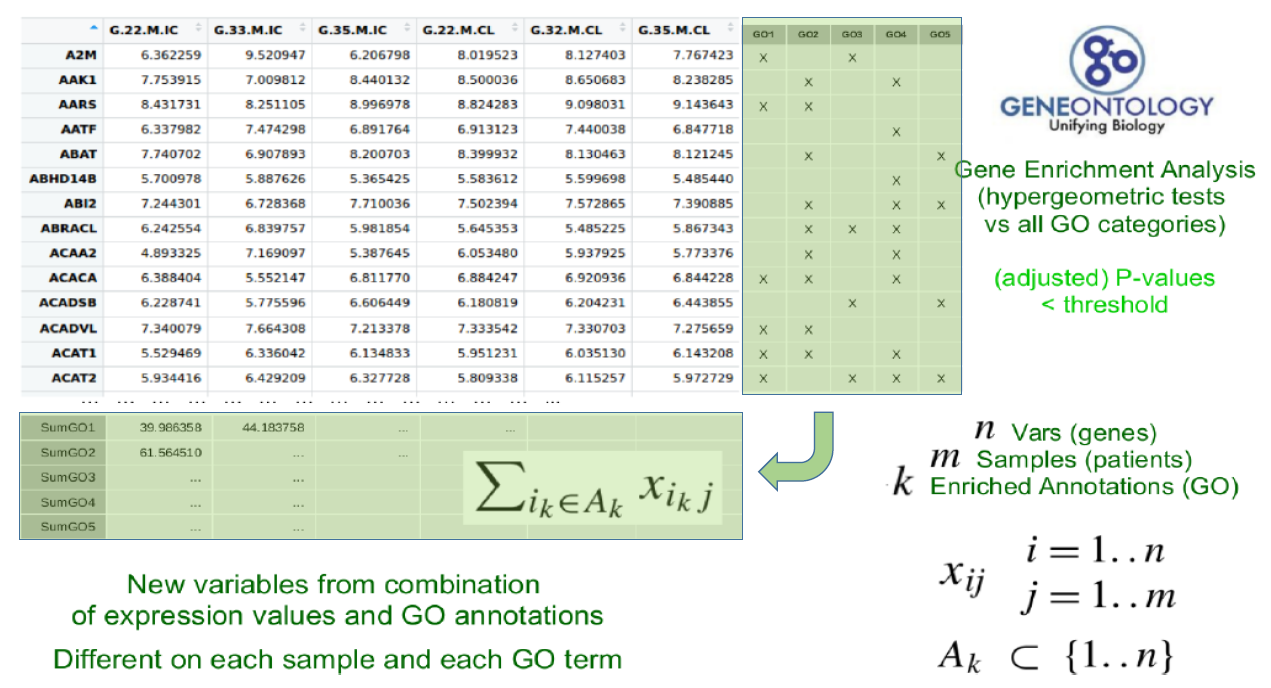
\includegraphics[width=0.95\linewidth]{figures/chapter3/3-1_addition_of_GO_terms} 

}

\caption{Addition of GO terms}\label{fig:fig3-1}
\end{figure}

Alternatively, manual annotations can be provided (eg. GO terms, canonical pathways, or even annotation to custom entities) as an optional input file. {[}mostrar el format requerit{]}.

Other annotation methods can be implemented, as functions to be used by the main pipeline, if more complex methods for biological information addition are required.

{[}Mostrar el format final de les anotacions, com a matrius dels data sets amb anotacions binàries 1/0 com a columnes extra{]}

Once the annotations are already computed, mapping each feature of the input data set to the corresponding biological entity, they can be used to generate new features (as new rows), computing the average value {[}punt de millora: ¿funció de ponderació?{]} of the expression/intensity values from all original features being mapped to the annotated biological entities.

\begin{figure}

{\centering 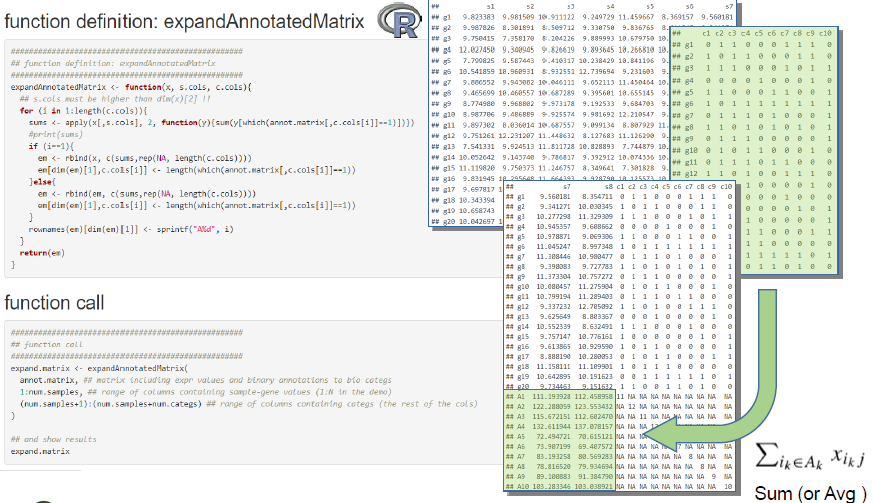
\includegraphics[width=0.95\linewidth]{figures/chapter3/3-2_addition_of_new_feats} 

}

\caption{Addition of news feats}\label{fig:fig3-2}
\end{figure}

\begin{figure}

{\centering 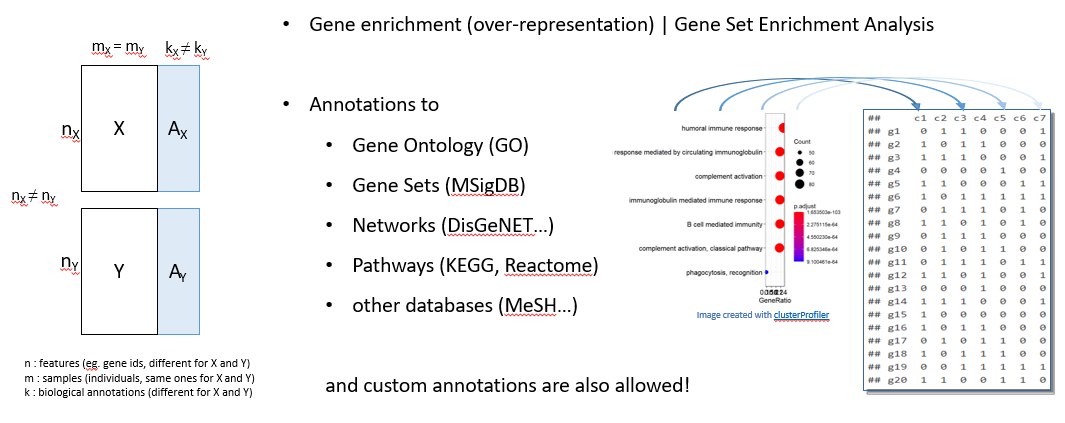
\includegraphics[width=0.95\linewidth]{figures/chapter3/3-3_gene_enrichment_diagram} 

}

\caption{Gene enrichment diagram}\label{fig:fig3-3}
\end{figure}

\begin{figure}

{\centering 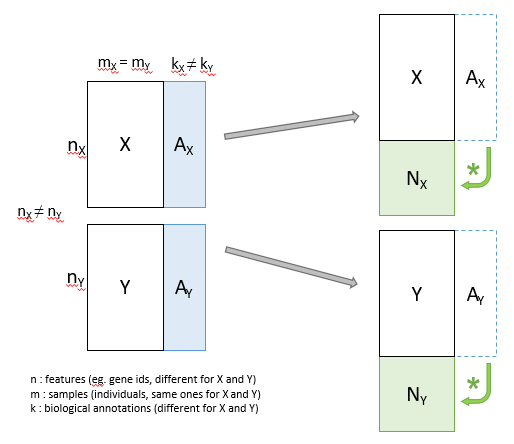
\includegraphics[width=0.95\linewidth]{figures/chapter3/3-4_matrix_expansion_diagram} 

}

\caption{Matrix expansion diagram}\label{fig:fig3-4}
\end{figure}

(Traduir) Una vez tenemos las matrices anotadas (Figura \ref{fig:fig3-4}, parte azul) pasamos a generar las matrices Expandidas (en verde) numerizando estas anotaciones, o sea, calculando la media de las expresiones numéricas de cada individuo para las variables anotadas a cada categoría. Esto se realiza con el producto matricial de los valores numéricos iniciales (expresion, proteinas\ldots) con las matrices traspuestas de sus anotaciones, y luego con la matriz inversa de una matriz diagonal del conteo de cuantas anotaciones ha tenido cada categoría o entidad anotada.

\begin{figure}

{\centering 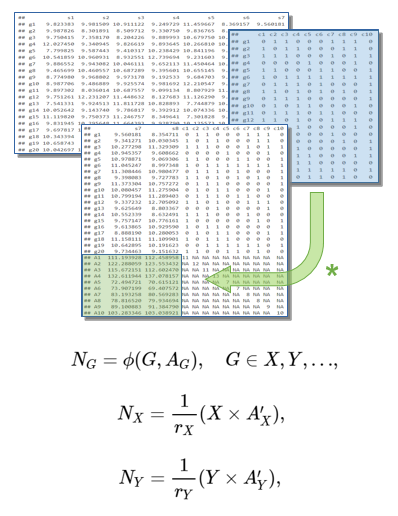
\includegraphics[width=0.95\linewidth]{figures/chapter3/3-5_addition_of_new_feats_2} 

}

\caption{Addition of new feats (2)}\label{fig:fig3-5}
\end{figure}

\begin{figure}

{\centering 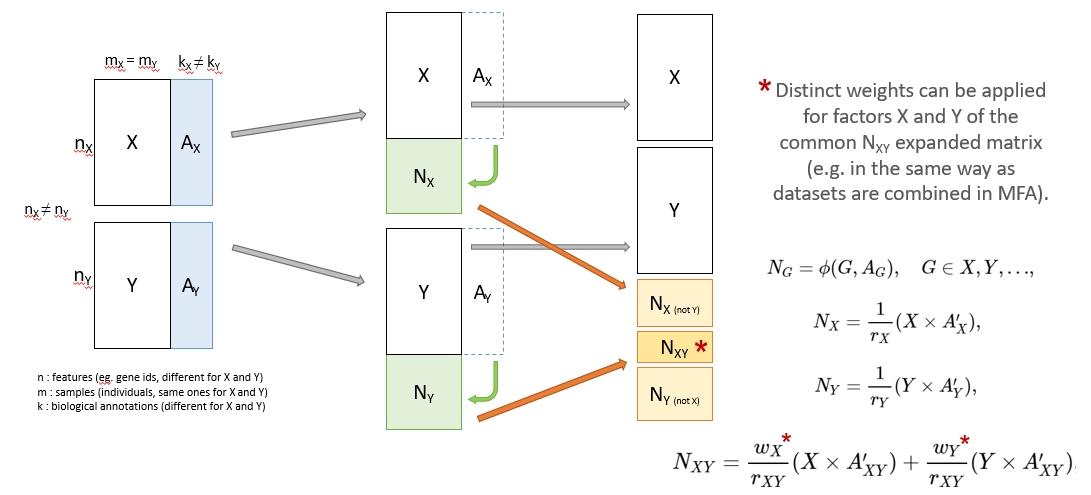
\includegraphics[width=0.95\linewidth]{figures/chapter3/3-6_matrix_expansion_diagram_2} 

}

\caption{Matrix expansion diagram (2)}\label{fig:fig3-6}
\end{figure}

\hypertarget{detail-of-the-integrative-data-analyses-applied}{%
\subsection{Detail of the integrative data analyses applied\ldots{}}\label{detail-of-the-integrative-data-analyses-applied}}

Mètodes:

1- Significació biològica, com faig les anotacions
2- Expansió de les matrius (creació de noves vars a partir de les anotacions)
3- Anàlisi factorial en detall, + MCIA + RGCCA
4- TFM sobre workflows i automatització -\textgreater{} Paquet targets en general

\hypertarget{comparison-of-oda-results}{%
\subsection{Comparison of ODA results}\label{comparison-of-oda-results}}

\hypertarget{numeric-measurement}{%
\subsection{Numeric measurement}\label{numeric-measurement}}

\% variabilitat explicat segons la estructura de la intersecció de les 2 taules

\hypertarget{biological-interpretation}{%
\subsection{Biological interpretation}\label{biological-interpretation}}

\hypertarget{targets-pipeline-concept}{%
\subsection{Targets PIPELINE concept}\label{targets-pipeline-concept}}

R package creation\ldots{}

Sistema que hem aplicat per crear el pipeline amb Targets\ldots{}

\begin{figure}

{\centering 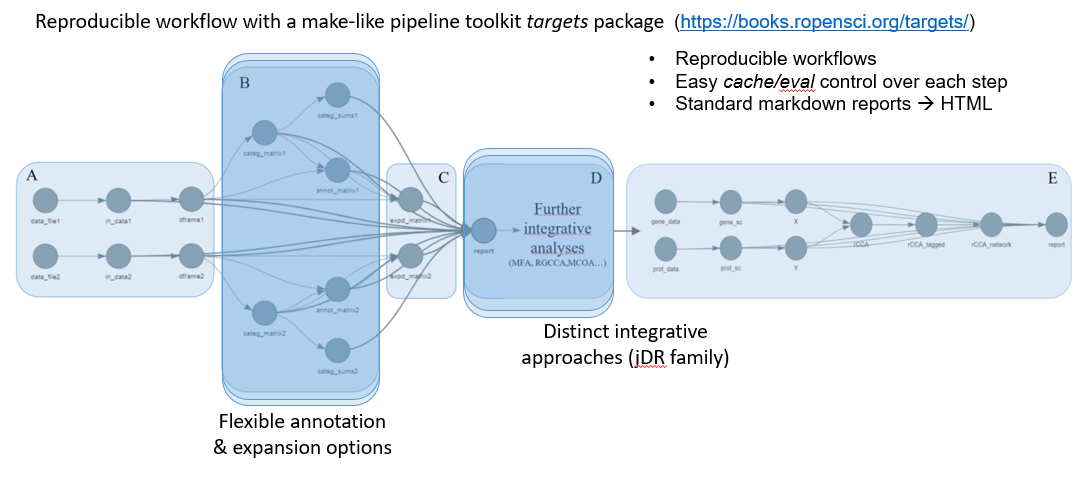
\includegraphics[width=0.95\linewidth]{figures/chapter3/3-7_workflow_overview} 

}

\caption{Workflow overview}\label{fig:fig3-7}
\end{figure}

Targets workflow diagram (Figure \ref{fig:fig3-7}) showing the steps corresponding with the complete process: The pipeline starts from (A) a couple of 'omics-derived input data sets (e.g.~pre-processed gene expression and protein abundance matrices). These are converted to R data frames with features in rows and samples in columns. Then, a data frame containing related annotations (B) is created, or loaded, for each given input matrix, and used to expand these original data, in order to end up with a pair of data frames (C) containing the original values plus the average expression/abundance values of the features related to each annotation as new features in additional rows. After that, distinct Dimension Reduction Methods are applied to perform the integrative analysis (D), and finally, an R markdown report (E) is rendered to show steps and main results of the full process.

\hypertarget{results}{%
\chapter{Results}\label{results}}

\chaptermark{Results}

\minitoc 

Text de presentacio dels resultats\ldots{}

\hypertarget{results-from-the-analysis-of-human-brain-tissue-samples}{%
\section{Results from the analysis of human brain tissue samples}\label{results-from-the-analysis-of-human-brain-tissue-samples}}

\hypertarget{results-from-the-expansion-of-omics-data-with-biological-annotations}{%
\section{Results from the expansion of omics data with biological annotations}\label{results-from-the-expansion-of-omics-data-with-biological-annotations}}

Figure \ref{fig:fig4-1} is an snapshot (F) of one of the heat maps created to show the expanded matrices obtained in (Figures \ref{fig:fig3-4} i \ref{fig:fig3-5} prèvies, de Methods).

\begin{figure}

{\centering 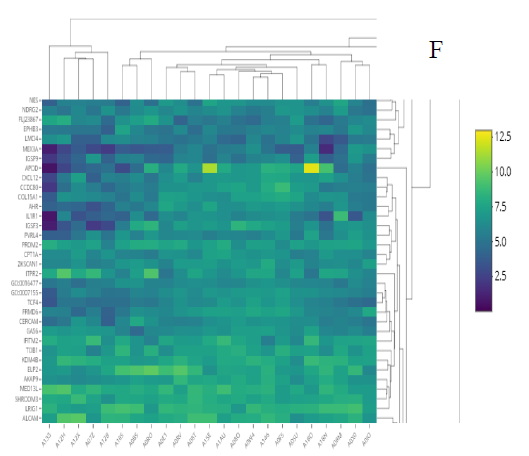
\includegraphics[width=0.95\linewidth]{figures/chapter4/4-1_heatmap_expanded} 

}

\caption{Heapmap of an expanded matrix}\label{fig:fig4-1}
\end{figure}

\hypertarget{results-from-the-analysis-of-150-tcga-brca-samples}{%
\section{Results from the analysis of 150 TCGA-BRCA samples}\label{results-from-the-analysis-of-150-tcga-brca-samples}}

Figure \ref{fig:fig4-2} contains some of the graphical results of the analysis of the 150 samples from TCGA-BRCA: Heat maps (A, C) and association networks (B, D) resulting from the integration by Regularized Canonical Correlations Analysis with mixomics R package. Performed with the original data sets (A, B) or using data expanded with biological annotations to Gene Ontology (C, D), so adding some GO terms to the features from each source, where the outputs contain higher level of information (higher density in both type of plots).

\begin{figure}

{\centering 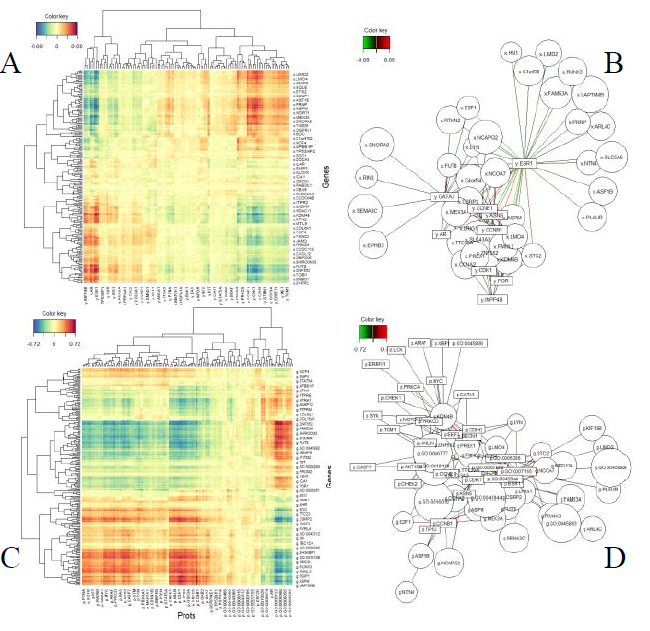
\includegraphics[width=0.95\linewidth]{figures/chapter4/4-2_BRCA_results_overview} 

}

\caption{BRCA results overview}\label{fig:fig4-2}
\end{figure}

\hypertarget{results-from-the-application-of-mfa-on-tcga-brca-data-with-and-without-expanded-data}{%
\section{Results from the application of MFA on TCGA-BRCA data with, and without, expanded data}\label{results-from-the-application-of-mfa-on-tcga-brca-data-with-and-without-expanded-data}}

Figure \ref{fig:fig4-3} includes a Correlation Circle (left), with most relevant genes, proteins and added GO annotations. Distribution of samples (right) along the first two plotted dimensions. Both results coming from the application of Multiple Factor Analysis (FactoMineR and factoextra R packages) performed on the same 150 samples (Basal, Her2 and LuminalA conditions) from TCGA-BRCA.

\begin{figure}

{\centering 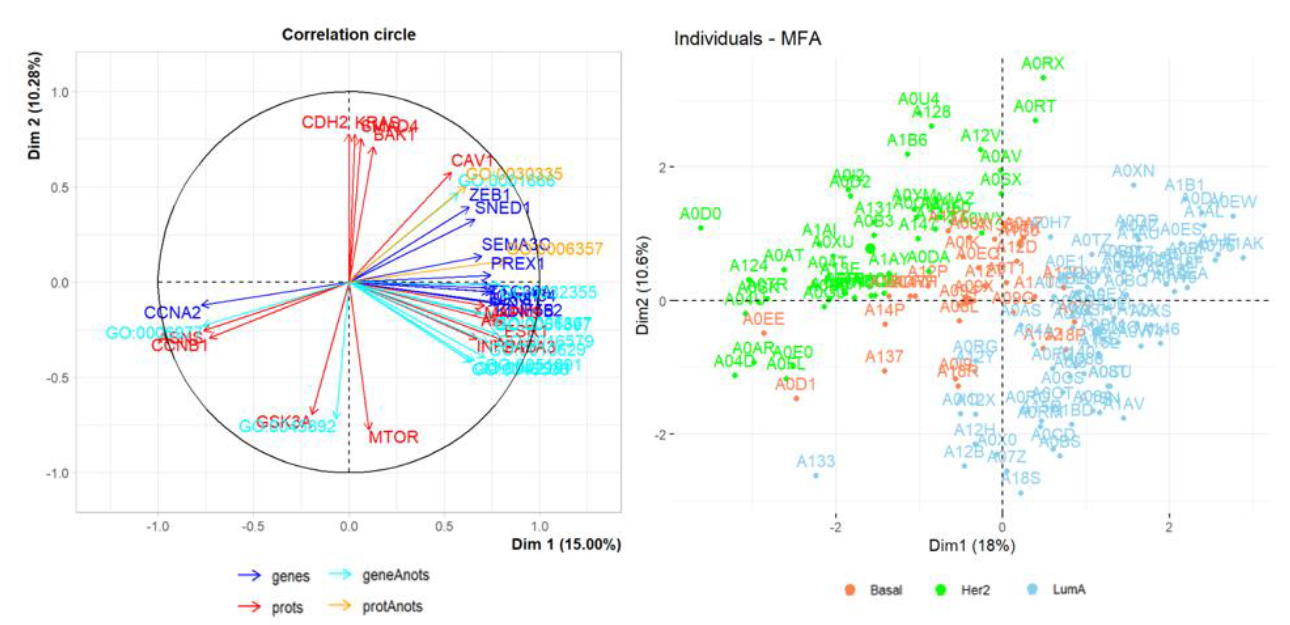
\includegraphics[width=0.95\linewidth]{figures/chapter4/4-3_BRCA_results_withMFA} 

}

\caption{BRCA results with MFA}\label{fig:fig4-3}
\end{figure}

\hypertarget{resultats-de-la-creacio-del-paquet-amb-targets}{%
\section{Resultats de la creacio del paquet amb Targets\ldots{}}\label{resultats-de-la-creacio-del-paquet-amb-targets}}

\clearpage

\hypertarget{discussion}{%
\chapter{Discussion}\label{discussion}}

\chaptermark{Discussion}

\minitoc 

Potser no cal posar la TOC aqui¿?

Resum de l'article. Apuntant a les conclusions. Comentant problemes i limitacions (emprar combinacions lineals de variables per crear-ne de noves).

Possibles extensions {[}punts de millora{]} Comentar i descriure cadascun d'ells:

\begin{itemize}
\tightlist
\item
  Poder fer servir 3 o més conjunts de dades
\item
  Poder ponderar els pesos de les anotacions, segons tipus, data set d'origen, etc.
\item
  Permetre treballar amb dades faltants o, fins i tot, blocs de dades faltants.
\item
  Millorar les opcions del paquet: mètodes d'anotació bio, mètodes d'integració, tipus de gràfics resultants\ldots{}
\end{itemize}

\begin{savequote}
There is grandeur in this view of life, with its several powers, having
been originally breathed into a few forms or into one; and that, whilst
this planet has gone cycling on according to the fixed law of gravity,
from so simple a beginning endless forms most beautiful and most
wonderful have been, and are being, evolved.
\qauthor{--- Charles Darwin (\protect\hyperlink{ref-Darwin1859}{\textbf{Darwin1859?}})}\end{savequote}



\hypertarget{conclusions}{%
\chapter{Conclusions}\label{conclusions}}

\chaptermark{Conclusions}

If we don't want Conclusion to have a chapter number next to it, we can add the \texttt{\{-\}} attribute.

\hypertarget{conclusion-1}{%
\section*{Conclusion 1}\label{conclusion-1}}
\addcontentsline{toc}{section}{Conclusion 1}

The need for a better biological interpretation of multi-omics integrative methods let us to consider the inclusion of biological information during (not after) the analysis process

\hypertarget{conclusion-2}{%
\section*{Conclusion 2}\label{conclusion-2}}
\addcontentsline{toc}{section}{Conclusion 2}

We propose a method focused on the expansion of the starting omics datasets, by adding new annotation-derived features to those matrices, before applying the integrative analysis

\hypertarget{conclusion-3}{%
\section*{Conclusion 3}\label{conclusion-3}}
\addcontentsline{toc}{section}{Conclusion 3}

This approach allows the inclusion of relevant information from the main biological annotation tools, as well as any custom annotation, combined with the use our preferred Dimension Reduction techniques

\hypertarget{conclusion-4}{%
\section*{Conclusion 4}\label{conclusion-4}}
\addcontentsline{toc}{section}{Conclusion 4}

We have implemented a pipeline for reproducible and easy-to-use execution, that facilitates the control of each step, the visualization of results and their reporting to PDF/HTML formats.

\startappendices

\hypertarget{the-first-appendix}{%
\chapter{The First Appendix}\label{the-first-appendix}}

This first appendix includes an R chunk that was hidden in the document (using \texttt{echo\ =\ FALSE}) to help with readibility:

\textbf{In 02-rmd-basics-code.Rmd}

\textbf{And here's another one from the same chapter, i.e.~Chapter \ref{code}:}

\hypertarget{the-second-appendix-for-fun}{%
\chapter{The Second Appendix, for Fun}\label{the-second-appendix-for-fun}}

\hypertarget{references}{%
\chapter*{References}\label{references}}
\addcontentsline{toc}{chapter}{References}

\markboth{References}{}

\hypertarget{refs}{}
\begin{CSLReferences}{1}{0}
\leavevmode\vadjust pre{\hypertarget{ref-cavill_transcriptomic_2016}{}}%
Cavill, R., Jennen, D., Kleinjans, J., \& Briedé, J. J. (2016). Transcriptomic and metabolomic data integration. \emph{Briefings in Bioinformatics}, \emph{17}(5), 891--901. \url{https://doi.org/10.1093/bib/bbv090}

\leavevmode\vadjust pre{\hypertarget{ref-meng_dimension_2016}{}}%
Meng, C., Zeleznik, O. A., Thallinger, G. G., Kuster, B., Gholami, A. M., \& Culhane, A. C. (2016). Dimension reduction techniques for the integrative analysis of multi-omics data. \emph{Briefings in Bioinformatics}, \emph{17}(4), 628--641. \url{https://doi.org/10.1093/bib/bbv108}

\leavevmode\vadjust pre{\hypertarget{ref-de_tayrac_simultaneous_2009}{}}%
Tayrac, M. de, Lê, S., Aubry, M., Mosser, J., \& Husson, F. (2009). Simultaneous analysis of distinct {Omics} data sets with integration of biological knowledge: {Multiple} {Factor} {Analysis} approach. \emph{BMC Genomics}, \emph{10}(1), 32. \url{https://doi.org/10.1186/1471-2164-10-32}

\end{CSLReferences}

%%%%% REFERENCES


\end{document}
